\documentclass[../competing_bandits.tex]{subfiles}
\begin{document}

\subsection{Performance in Isolation}\label{sec:isolation}

We start with a pilot experiment in which we investigate each algorithm's performance ``in isolation": in a stand-alone MAB problem without competition. We focus on reputation scores generated by each algorithm. We confirm that algorithms' performance is ordered as we'd expect:
    $\TS > \DEG > \DG$
for a sufficiently long time horizon. For each algorithm and each MAB instance, we compute the mean reputation score at each round, averaged over all \MRVs. We plot the \emph{mean reputation trajectory}: how this score evolves over time. Figure \ref{prelim_means} shows such a plot for the Needle-in-Haystack instance; for other MAB instances the plots are similar. We summarize this finding as follows:

\begin{finding}
\textit{The mean reputation trajectories are arranged as predicted by prior work:
    $\TS > \DEG > \DG$ for a sufficiently long time horizon.}
\end{finding}


\begin{figure}
\centering
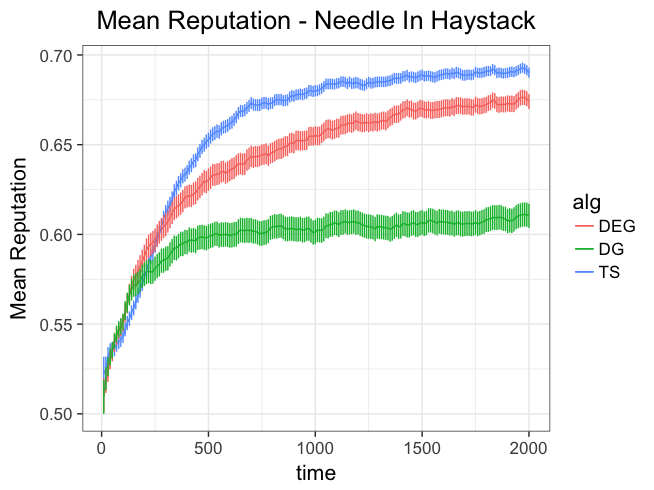
\includegraphics[scale=0.3]{ec19paper/figures/nih_iso_mean}
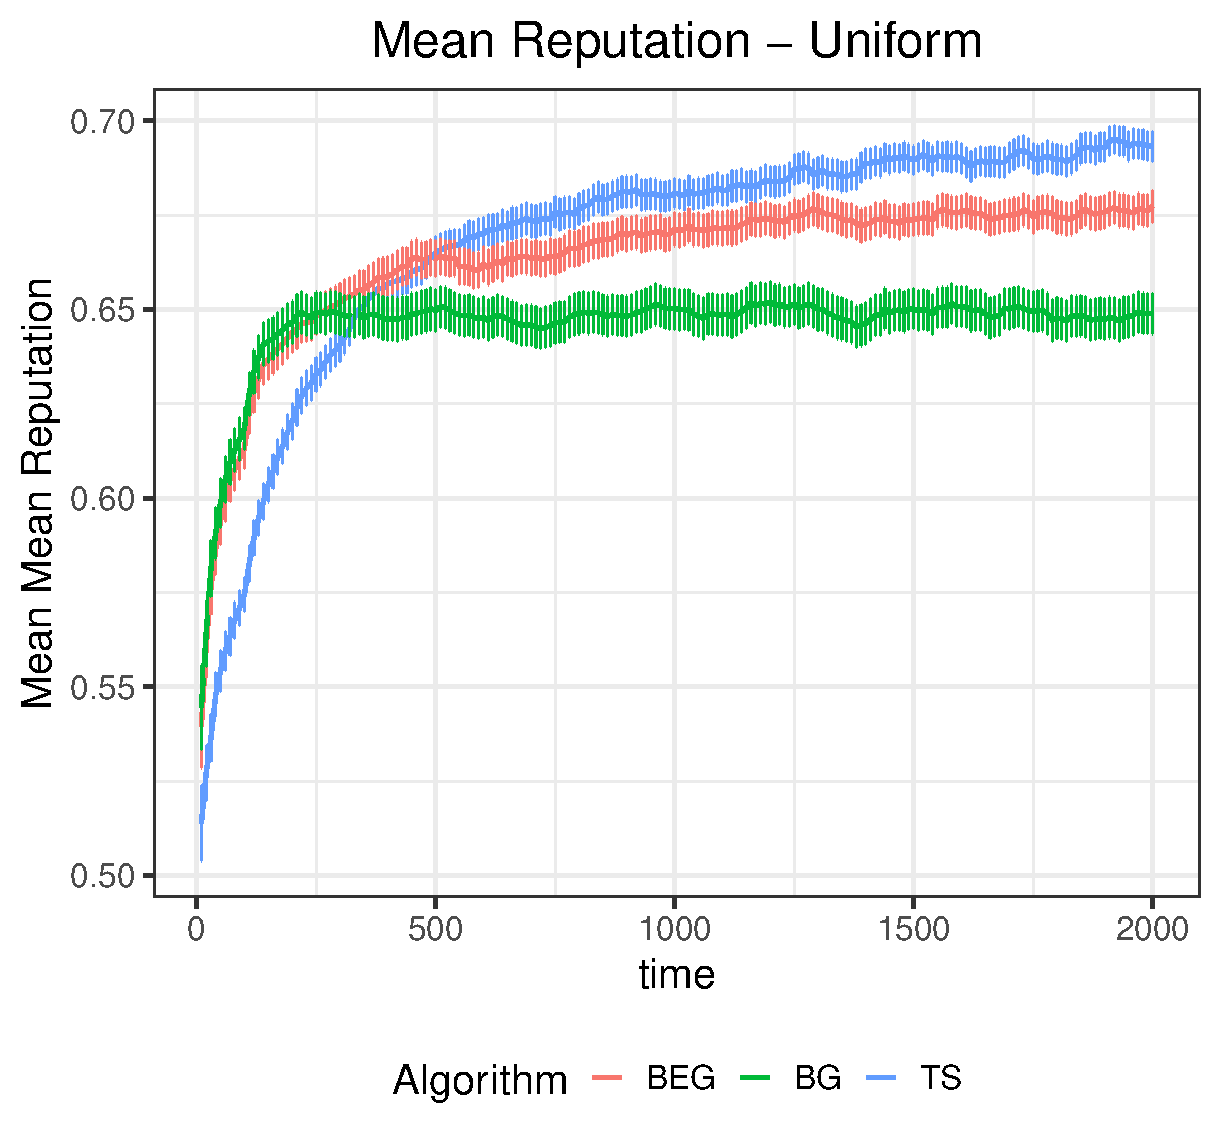
\includegraphics[scale=0.4]{ec19paper/appendix_figures/uniform_mean}
%\caption*{\tiny{Mean reputation trajectory The plots contain the average reputation over $1000$ runs for a memory size of $100$ where, for a given $t$, we record the reputation of a given algorithm on a given instance and then average this value across all the runs. The shaded area display 95\% confidence intervals.}}
\caption{Mean reputation trajectories for Needle-in-Haystack and Uniform. The shaded area shows 95\% confidence intervals.}
\label{prelim_means}
\end{figure}

We also use Figure~\ref{prelim_means} to choose a reasonable time-horizon for the subsequent experiments, as $T=2000$. The idea is, we want $T$ to be large enough so that algorithms performance starts to plateau, but small enough such that algorithms are still learning.

The mean reputation trajectory is probably the most natural way to represent an algorithm's performance on a given MAB instance. However, we found that the outcomes of the competition game are better explained with a different ``performance-in-isolation" statistic that is more directly connected to the game. Consider the  performance of two algorithms, Alg1 and Alg2, ``in isolation" on a particular MAB instance. The \emph{relative reputation} of Alg1 (vs. Alg2) at a given time $t$ is the fraction of \MRVs /realization tables for which Alg1 has a higher reputation score than Alg2. The intuition is that agent's selection in our model depends only on the comparison between the reputation scores.

\begin{figure}[ht]
\centering
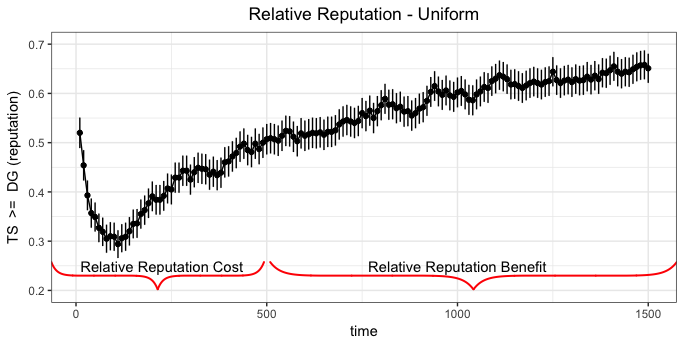
\includegraphics[scale=0.35]{ec19paper/figures/relative_uniform_annotated_plot}
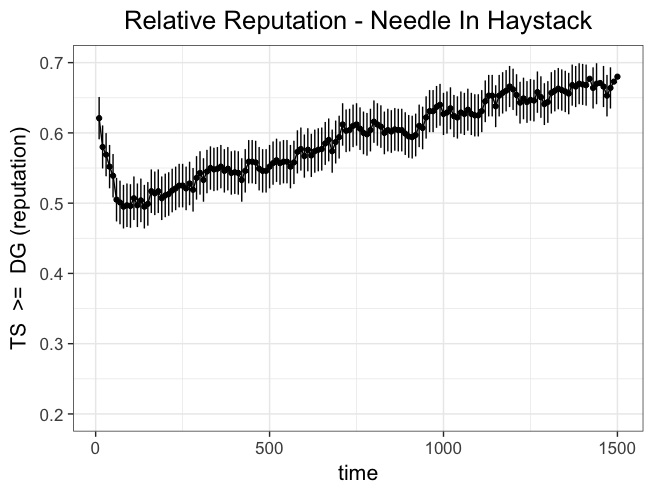
\includegraphics[scale=0.35]{ec19paper/figures/relative_nih_ts_dg.png}
%\caption*{\tiny{The plots contain the average reputation over $1000$ runs for a memory size of $100$ where, for a given $t$, we record the reputation of both of the algorithms on a given instance and then calculate the proportion of runs where $\TS \geq \DG$. The shaded area display 95\% confidence intervals.}}
\caption{Relative reputation trajectory for $\TS$ vs $\DG$, on Uniform instance (top) and Needle-in-Haystack instance (bottom). Shaded area display 95\% confidence intervals.}
\label{relative_rep_plots}
\end{figure}

This angle allows a more nuanced analysis of reputation costs vs. benefits under competition. Figure \ref{relative_rep_plots} (top) shows the relative reputation trajectory for $\TS$ vs $\DG$ for the Uniform instance. The relative reputation is less than $\tfrac12$ in the early rounds, meaning that $\DG$ has a higher reputation score in a majority of the simulations, and more than $\tfrac12$ later on. The reason is the exploration in \TS leads to worse decisions initially, but allows for better decisions later. The time period when relative reputation vs. \DG dips below $\tfrac12$ can be seen as an explanation for the competitive disadvantage of exploration. Such period also exists for the Heavy-Tail MAB instance. However, it does not exist for the Needle-in-Haystack instance, see Figure \ref{relative_rep_plots} (bottom).%
\footnote{We see two explanations for this: $\TS$ identifies the best arm faster for the Needle-in-Haystack instance, and there are no ``very bad" arms which make exploration very expensive in the short term.}


\begin{finding}\label{find:period}
\textit{Exploration can lead to relative reputation vs. $\DG$ going below $\tfrac12$ for some initial time period. This happens for some MAB instances but not for some others.}
\end{finding}

\begin{definition}
For a particular MAB algorithm, a time period when relative reputation vs. \DG goes below $\tfrac12$ is called {\em exploration disadvantage period}. An MAB instance is called \emph{exploration-disadvantaged} if such period exists.
\end{definition}

\noindent Uniform and Heavy-tail instance are exploration-disadvantaged, but Needle-in-Haystack is not.

\end{document} 